%
% File acl2017.tex
%
%% Based on the style files for ACL-2015, with some improvements
%%  taken from the NAACL-2016 style
%% Based on the style files for ACL-2014, which were, in turn,
%% based on ACL-2013, ACL-2012, ACL-2011, ACL-2010, ACL-IJCNLP-2009,
%% EACL-2009, IJCNLP-2008...
%% Based on the style files for EACL 2006 by 
%%e.agirre@ehu.es or Sergi.Balari@uab.es
%% and that of ACL 08 by Joakim Nivre and Noah Smith

\documentclass[11pt,a4paper]{article}
\usepackage[hyperref]{acl2017}
\usepackage{graphicx}
\usepackage{times}
\usepackage{latexsym}

\usepackage{url}

\aclfinalcopy % Uncomment this line for the final submission
%\def\aclpaperid{***} %  Enter the acl Paper ID here

%\setlength\titlebox{5cm}
% You can expand the titlebox if you need extra space
% to show all the authors. Please do not make the titlebox
% smaller than 5cm (the original size); we will check this
% in the camera-ready version and ask you to change it back.

\newcommand\BibTeX{B{\sc ib}\TeX}

\title{ %
  Congestion-Control Algorithms on an Emulated Cellular Network\\
\large CS 244 PA2 Writeup}

\author{Hope Casey-Allen  \\
  {\tt hcaseyal@stanford.edu} \\\And
  Jiaxin Guan \\
  {\tt jxguan@stanford.edu} \\}

\date{}

\begin{document}
\maketitle
\begin{abstract}
  This document contains the instructions for preparing a camera-ready
  manuscript for the proceedings of ACL-2017. The document itself
  conforms to its own specifications, and is therefore an example of
  what your manuscript should look like. These instructions should be
  used for both papers submitted for review and for final versions of
  accepted papers.  Authors are asked to conform to all the directions
  reported in this document.
\end{abstract}



\section{Fixed Window Size}

\subsection{Varying the Window Sizes}
We created a script to vary the fixed window size and output results for average
capacity, average throughput, 95th percentile per-packet queueing delay, and
95th percentile signal delay (see \texttt{datagrump/warmup-a.sh}). We took measurements
with windows sizes of $1$, $2$, $5$, $10$, $20$, $50$, $100$, $200$, $500$ and
took them over $3$ runs
each to estimate the repeatability of the measurements. The results we had are
shown in figure \ref{fig:warmup-a}.
\begin{figure}[h]
  \centering
  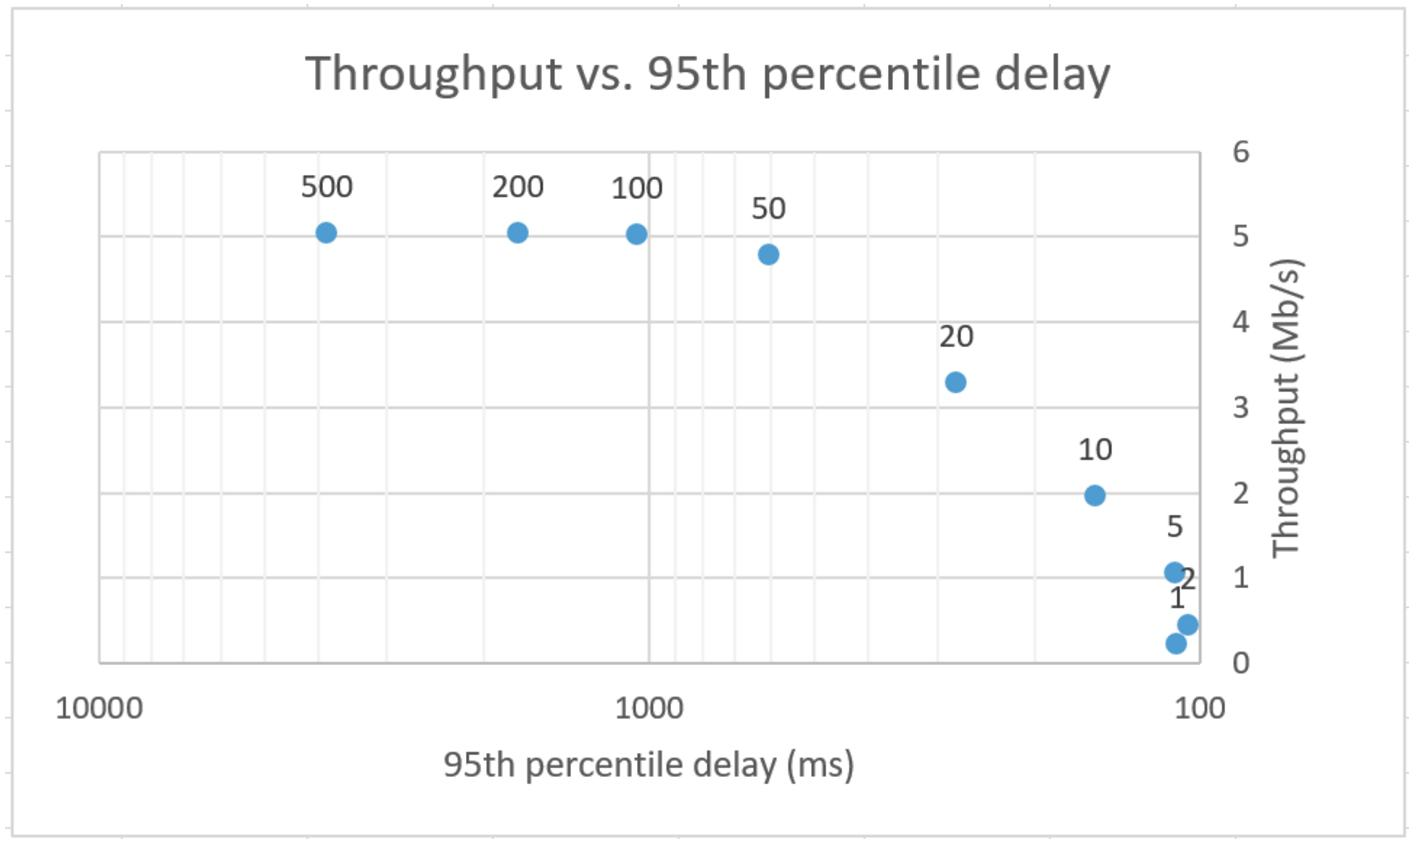
\includegraphics[scale=0.15]{warmup-a}
  \caption{The performance for different fixed window sizes. Data Labels
  represent the corresponding fixed window size.}
  \label{fig:warmup-a}
\end{figure}

We can observe an overall pattern that by increasing the window size, we're able
to obtain better network utilization, but at the same time getting higher delay.
This matches our expectation as we would expect the queue to be full and the
network fully utilized for large fixed window sizes.

Another interesting observation is that when increasing the window size
from $1$ to $2$, the throughput increases, while at the same time the delay also
slightly decreases. This is interesting in that normally we would expect the
delay to increase as we increase the window size. We suspect that it is because
with a
larger window size $2$, which is still way smaller than the network capacity, more
packets can be sent through the network when the network is not at all
congested. In this way, we have more packets with low delay for window size $2$,
and hence a lower average delay.

Notice that this reasoning only applies
to window sizes that are way smaller than the max network capacity, because with
relatively large window sizes, the network is likely often fully utilized -
increasing the window size would not lead to more packets being delivered with
low delay, but rather it will lead to more packets waiting in the queue when the
network is congested, and hence a higher average delay.

\subsection{Best Fixed Window Size}
By examining the
results from section $1.1$, we observed that the window size that maximized the
overall score was between $5$
and $20$. 
We then reran the script, but this time varying the input window size
parameter between $5$ and 
$20$ to perform a ternary search to find the exact best window
size. The resulting best fixed window size that we found is $12$, with a score of
$12.84$ using the $\text{throughput}/\text{delay}$ function on the contest page (or
$3.68$ if using the $\log(\text{throughput}/\text{delay})$  function on the assignment
handout).
This is not a great result, but it is more than $10$ times better than
the performance for fixed window size $1$.

\subsection{Repeatability}

We calculated the standard deviation for our results for the best fixed window
size over $10$ runs (see table \ref{tab:warmup-a}). We can see that the standard
deviations are very low when compared to the averages, showing that the
measurements are extremely repeatable. This matches our expectation because
all of the code is deterministic. The only source of variations is the
fluctuation of the machine performance.

\begin{table}
  \centering
  \begin{tabular}{|c|r|r|}
    \hline
                         & \multicolumn{1}{c|}{StdDev} &
    \multicolumn{1}{c|}{Avg} \\ \hline
    Throughput (Mbits/s) & 0.005                       & 2.263
    \\ \hline
    Delay (ms)           & 0.333                       & 175.889
    \\ \hline
    Score                & 0.046                       & 12.868
    \\ \hline
  \end{tabular}
  \caption{The standard deviations and averages of the throughput, delay and
  overall score.}
  \label{tab:warmup-a}
\end{table}

\section{Additive Increase, Multiplicative Decrease}

\subsection{Implementation}

We implemented the AIMD scheme in \texttt{datagrump/controller.cc}. We made a slight modification that we perform
a multiplicative decrease whenever the RTT exceeds a specific timeout. This
simulates the situations where packets get lost in transmission and are resent
after a timeout (conventionally $2* RTT$). We derived the actual RTT by using
the timestamps in the \texttt{ack\_received} function per the Piazza post. We
tested the implementation first with arbitrarily set constants, which gave us a score
around $18$, which is a significant improvement over the fixed window size
algorithm.

\subsection{Choosing the Constants}

In order to choose the constants that yield the best performance, we wrote a
script to try different constants of initial window size, additive increase
size, and multiplicative decrease factor. We were able to get the result shown
in table \ref{tab:warmup-b}

\begin{table}[]
  \centering
  \label{tab:warmup-b}
  \begin{tabular}{|c|r|r|r|r|r|}
    \hline
    \multicolumn{1}{|l|}{} & \multicolumn{1}{c|}{1} & \multicolumn{1}{c|}{2} &
    \multicolumn{1}{c|}{4} & \multicolumn{1}{c|}{8} & \multicolumn{1}{c|}{16} \\
    \hline
    0.2                    & 18.52                  & 18.55                  &
    14.97                  & 12.91                  & 10.65                   \\
    \hline
    0.4                    & 18.81                  & 18.75                  &
    14.74                  & 12.79                  & 11.06                   \\
    \hline
    0.6                    & 17.37                  & 18.67                  &
    14.95                  & 12.98                  & 10.63                   \\
    \hline
    0.8                    & 17.99                  & 18.33                  &
    15.30                  & 13.24                  & 10.76                   \\
    \hline
  \end{tabular}
  \caption{Blahblahblah}
\end{table}


\section{General Instructions}

Manuscripts must be in two-column format.  Exceptions to the
two-column format include the title, authors' names and complete
addresses, which must be centered at the top of the first page, and
any full-width figures or tables (see the guidelines in
Subsection~\ref{ssec:first}). {\bf Type single-spaced.}  Start all
pages directly under the top margin. See the guidelines later
regarding formatting the first page.  The manuscript should be
printed single-sided and its length
should not exceed the maximum page limit described in Section~\ref{sec:length}.
Pages are numbered for  initial submission. However, {\bf do not number the pages in the camera-ready version}.

By uncommenting {\small\verb|\aclfinalcopy|} at the top of this 
 document, it will compile to produce an example of the camera-ready formatting; by leaving it commented out, the document will be anonymized for initial submission.  When you first create your submission on softconf, please fill in your submitted paper ID where {\small\verb|***|} appears in the {\small\verb|\def\aclpaperid{***}|} definition at the top.

The review process is double-blind, so do not include any author information (names, addresses) when submitting a paper for review.  
However, you should maintain space for names and addresses so that they will fit in the final (accepted) version.  The ACL 2017 \LaTeX\ style will create a titlebox space of 2.5in for you when {\small\verb|\aclfinalcopy|} is commented out.  

\subsection{The Ruler}
The ACL 2017 style defines a printed ruler which should be presented in the
version submitted for review.  The ruler is provided in order that
reviewers may comment on particular lines in the paper without
circumlocution.  If you are preparing a document without the provided
style files, please arrange for an equivalent ruler to
appear on the final output pages.  The presence or absence of the ruler
should not change the appearance of any other content on the page.  The
camera ready copy should not contain a ruler. (\LaTeX\ users may uncomment
the {\small\verb|\aclfinalcopy|} command in the document preamble.)  

Reviewers: note that the ruler measurements do not align well with
lines in the paper -- this turns out to be very difficult to do well
when the paper contains many figures and equations, and, when done,
looks ugly. In most cases one would expect that the approximate
location will be adequate, although you can also use fractional
references ({\em e.g.}, the first paragraph on this page ends at mark $114.5$).

\subsection{Electronically-available resources}

ACL provides this description in \LaTeX2e{} ({\small\tt acl2017.tex}) and PDF
format ({\small\tt acl2017.pdf}), along with the \LaTeX2e{} style file used to
format it ({\small\tt acl2017.sty}) and an ACL bibliography style ({\small\tt acl\_natbib.bst})
and example bibliography ({\small\tt acl2017.bib}).
These files are all available at
{\small\tt acl2017.org/index.php?article\_id=9}. We
strongly recommend the use of these style files, which have been
appropriately tailored for the ACL 2017 proceedings.

\subsection{Format of Electronic Manuscript}
\label{sect:pdf}

For the production of the electronic manuscript you must use Adobe's
Portable Document Format (PDF). PDF files are usually produced from
\LaTeX\ using the \textit{pdflatex} command. If your version of
\LaTeX\ produces Postscript files, you can convert these into PDF
using \textit{ps2pdf} or \textit{dvipdf}. On Windows, you can also use
Adobe Distiller to generate PDF.

Please make sure that your PDF file includes all the necessary fonts
(especially tree diagrams, symbols, and fonts with Asian
characters). When you print or create the PDF file, there is usually
an option in your printer setup to include none, all or just
non-standard fonts.  Please make sure that you select the option of
including ALL the fonts. \textbf{Before sending it, test your PDF by
  printing it from a computer different from the one where it was
  created.} Moreover, some word processors may generate very large PDF
files, where each page is rendered as an image. Such images may
reproduce poorly. In this case, try alternative ways to obtain the
PDF. One way on some systems is to install a driver for a postscript
printer, send your document to the printer specifying ``Output to a
file'', then convert the file to PDF.

It is of utmost importance to specify the \textbf{A4 format} (21 cm
x 29.7 cm) when formatting the paper. When working with
{\tt dvips}, for instance, one should specify {\tt -t a4}.
Or using the command \verb|\special{papersize=210mm,297mm}| in the latex
preamble (directly below the \verb|\usepackage| commands). Then using 
{\tt dvipdf} and/or {\tt pdflatex} which would make it easier for some.

Print-outs of the PDF file on A4 paper should be identical to the
hardcopy version. If you cannot meet the above requirements about the
production of your electronic submission, please contact the
publication chairs as soon as possible.

\subsection{Layout}
\label{ssec:layout}

Format manuscripts two columns to a page, in the manner these
instructions are formatted. The exact dimensions for a page on A4
paper are:

\begin{itemize}
\item Left and right margins: 2.5 cm
\item Top margin: 2.5 cm
\item Bottom margin: 2.5 cm
\item Column width: 7.7 cm
\item Column height: 24.7 cm
\item Gap between columns: 0.6 cm
\end{itemize}

\noindent Papers should not be submitted on any other paper size.
 If you cannot meet the above requirements about the production of 
 your electronic submission, please contact the publication chairs 
 above as soon as possible.

\subsection{Fonts}

For reasons of uniformity, Adobe's {\bf Times Roman} font should be
used. In \LaTeX2e{} this is accomplished by putting

\begin{quote}
\begin{verbatim}
\usepackage{times}
\usepackage{latexsym}
\end{verbatim}
\end{quote}
in the preamble. If Times Roman is unavailable, use {\bf Computer
  Modern Roman} (\LaTeX2e{}'s default).  Note that the latter is about
  10\% less dense than Adobe's Times Roman font.

\begin{table}[h]
\begin{center}
\begin{tabular}{|l|rl|}
\hline \bf Type of Text & \bf Font Size & \bf Style \\ \hline
paper title & 15 pt & bold \\
author names & 12 pt & bold \\
author affiliation & 12 pt & \\
the word ``Abstract'' & 12 pt & bold \\
section titles & 12 pt & bold \\
document text & 11 pt  &\\
captions & 11 pt & \\
abstract text & 10 pt & \\
bibliography & 10 pt & \\
footnotes & 9 pt & \\
\hline
\end{tabular}
\end{center}
\caption{\label{font-table} Font guide. }
\end{table}

\subsection{The First Page}
\label{ssec:first}

Center the title, author's name(s) and affiliation(s) across both
columns. Do not use footnotes for affiliations. Do not include the
paper ID number assigned during the submission process. Use the
two-column format only when you begin the abstract.

{\bf Title}: Place the title centered at the top of the first page, in
a 15-point bold font. (For a complete guide to font sizes and styles,
see Table~\ref{font-table}) Long titles should be typed on two lines
without a blank line intervening. Approximately, put the title at 2.5
cm from the top of the page, followed by a blank line, then the
author's names(s), and the affiliation on the following line. Do not
use only initials for given names (middle initials are allowed). Do
not format surnames in all capitals ({\em e.g.}, use ``Mitchell'' not
``MITCHELL'').  Do not format title and section headings in all
capitals as well except for proper names (such as ``BLEU'') that are
conventionally in all capitals.  The affiliation should contain the
author's complete address, and if possible, an electronic mail
address. Start the body of the first page 7.5 cm from the top of the
page.

The title, author names and addresses should be completely identical
to those entered to the electronical paper submission website in order
to maintain the consistency of author information among all
publications of the conference. If they are different, the publication
chairs may resolve the difference without consulting with you; so it
is in your own interest to double-check that the information is
consistent.

{\bf Abstract}: Type the abstract at the beginning of the first
column. The width of the abstract text should be smaller than the
width of the columns for the text in the body of the paper by about
0.6 cm on each side. Center the word {\bf Abstract} in a 12 point bold
font above the body of the abstract. The abstract should be a concise
summary of the general thesis and conclusions of the paper. It should
be no longer than 200 words. The abstract text should be in 10 point font.

{\bf Text}: Begin typing the main body of the text immediately after
the abstract, observing the two-column format as shown in 
the present document. Do not include page numbers.

{\bf Indent}: When starting a new paragraph. Use 11 points for text and 
subsection headings, 12 points for section headings and 15 points for
the title. 

\begin{table}
\centering
\small
\begin{tabular}{cc}
\begin{tabular}{|l|l|}
\hline
{\bf Command} & {\bf Output}\\\hline
\verb|{\"a}| & {\"a} \\
\verb|{\^e}| & {\^e} \\
\verb|{\`i}| & {\`i} \\ 
\verb|{\.I}| & {\.I} \\ 
\verb|{\o}| & {\o} \\
\verb|{\'u}| & {\'u}  \\ 
\verb|{\aa}| & {\aa}  \\\hline
\end{tabular} & 
\begin{tabular}{|l|l|}
\hline
{\bf Command} & {\bf  Output}\\\hline
\verb|{\c c}| & {\c c} \\ 
\verb|{\u g}| & {\u g} \\ 
\verb|{\l}| & {\l} \\ 
\verb|{\~n}| & {\~n} \\ 
\verb|{\H o}| & {\H o} \\ 
\verb|{\v r}| & {\v r} \\ 
\verb|{\ss}| & {\ss} \\\hline
\end{tabular}
\end{tabular}
\caption{Example commands for accented characters, to be used in, {\em e.g.}, \BibTeX\ names.}\label{tab:accents}
\end{table}

\subsection{Sections}

{\bf Headings}: Type and label section and subsection headings in the
style shown on the present document.  Use numbered sections (Arabic
numerals) in order to facilitate cross references. Number subsections
with the section number and the subsection number separated by a dot,
in Arabic numerals. Do not number subsubsections.

\begin{table*}
\centering
\begin{tabular}{lll}
  output & natbib & previous ACL style files\\
  \hline
  \citep{Gusfield:97} & \verb|\citep| & \verb|\cite| \\
  \citet{Gusfield:97} & \verb|\citet| & \verb|\newcite| \\
  \citeyearpar{Gusfield:97} & \verb|\citeyearpar| & \verb|\shortcite| \\
\end{tabular}
\caption{Citation commands supported by the style file.
  The citation style is based on the natbib package and
  supports all natbib citation commands.
  It also supports commands defined in previous ACL style files
  for compatibility.
  }
\end{table*}

{\bf Citations}: Citations within the text appear in parentheses
as~\cite{Gusfield:97} or, if the author's name appears in the text
itself, as Gusfield~\shortcite{Gusfield:97}.
Using the provided \LaTeX\ style, the former is accomplished using
{\small\verb|\cite|} and the latter with {\small\verb|\shortcite|} or {\small\verb|\newcite|}.  Collapse multiple citations as in~\cite{Gusfield:97,Aho:72}; this is accomplished with the provided style using commas within the {\small\verb|\cite|} command, {\em e.g.}, {\small\verb|\cite{Gusfield:97,Aho:72}|}.  
Append lowercase letters to the year in cases of ambiguities.  
 Treat double authors as
in~\cite{Aho:72}, but write as in~\cite{Chandra:81} when more than two
authors are involved. Collapse multiple citations as
in~\cite{Gusfield:97,Aho:72}. Also refrain from using full citations
as sentence constituents.

\penalty -5000

We suggest that instead of
\begin{quote}
  ``\cite{Gusfield:97} showed that ...''
\end{quote}
you use
\begin{quote}
``Gusfield \shortcite{Gusfield:97}   showed that ...''
\end{quote}

If you are using the provided \LaTeX{} and Bib\TeX{} style files, you
can use the command \verb|\citet| (cite in text)
to get ``author (year)'' citations.

If the Bib\TeX{} file contains DOI fields, the paper
title in the references section will appear as a hyperlink
to the DOI, using the hyperref \LaTeX{} package.
To disable the hyperref package, load the style file
with the \verb|nohyperref| option:
\verb|\usepackage[nohyperref]{acl2017}|

\textbf{Digital Object Identifiers}:  As part of our work to make ACL
materials more widely used and cited outside of our discipline, ACL
has registered as a CrossRef member, as a registrant of Digital Object
Identifiers (DOIs), the standard for registering permanent URNs for
referencing scholarly materials.  As of 2017, we are requiring all
camera-ready references to contain the appropriate DOIs (or as a
second resort, the hyperlinked ACL Anthology Identifier) to all cited
works.  Thus, please ensure that you use Bib\TeX records that contain
DOI or URLs for any of the ACL materials that you reference.
Appropriate records should be found for most materials in the current
ACL Anthology at \url{http://aclanthology.info/}.

As examples, we cite \cite{P16-1001} to show you how papers with a DOI
will appear in the bibliography.  We cite \cite{C14-1001} to show how
papers without a DOI but with an ACL Anthology Identifier will appear
in the bibliography.  

As reviewing will be double-blind, the submitted version of the papers
should not include the authors' names and affiliations. Furthermore,
self-references that reveal the author's identity, {\em e.g.},
\begin{quote}
``We previously showed \cite{Gusfield:97} ...''  
\end{quote}
should be avoided. Instead, use citations such as 
\begin{quote}
``\citeauthor{Gusfield:97} \shortcite{Gusfield:97}
previously showed ... ''
\end{quote}

\textbf{Please do not use anonymous citations} and do not include
acknowledgements when submitting your papers. Papers that do not
conform to these requirements may be rejected without review.

\textbf{References}: Gather the full set of references together under
the heading {\bf References}; place the section before any Appendices,
unless they contain references. Arrange the references alphabetically
by first author, rather than by order of occurrence in the text.
Provide as complete a citation as possible, using a consistent format,
such as the one for {\em Computational Linguistics\/} or the one in the 
{\em Publication Manual of the American 
Psychological Association\/}~\cite{APA:83}.  Use of full names for
authors rather than initials is preferred.  A list of abbreviations
for common computer science journals can be found in the ACM 
{\em Computing Reviews\/}~\cite{ACM:83}.

The \LaTeX{} and Bib\TeX{} style files provided roughly fit the
American Psychological Association format, allowing regular citations, 
short citations and multiple citations as described above.

{\bf Appendices}: Appendices, if any, directly follow the text and the
references (but see above).  Letter them in sequence and provide an
informative title: {\bf Appendix A. Title of Appendix}.

\subsection{Footnotes}

{\bf Footnotes}: Put footnotes at the bottom of the page and use 9
points text. They may be numbered or referred to by asterisks or other
symbols.\footnote{This is how a footnote should appear.} Footnotes
should be separated from the text by a line.\footnote{Note the line
separating the footnotes from the text.}

\subsection{Graphics}

{\bf Illustrations}: Place figures, tables, and photographs in the
paper near where they are first discussed, rather than at the end, if
possible.  Wide illustrations may run across both columns.  Color
illustrations are discouraged, unless you have verified that  
they will be understandable when printed in black ink.

{\bf Captions}: Provide a caption for every illustration; number each one
sequentially in the form:  ``Figure 1. Caption of the Figure.'' ``Table 1.
Caption of the Table.''  Type the captions of the figures and 
tables below the body, using 11 point text.

\subsection{Accessibility}
\label{ssec:accessibility}

In an effort to accommodate the color-blind (as well as those printing
to paper), grayscale readability for all accepted papers will be
encouraged.  Color is not forbidden, but authors should ensure that
tables and figures do not rely solely on color to convey critical
distinctions.
Here we give a simple criterion on your colored figures, if your paper has to be printed in black and white, then you must assure that every curves or points in your figures can be still clearly distinguished.

% Min: no longer used as of ACL 2017, following ACL exec's decision to
% remove this extra workflow that was not executed much.
% BEGIN: remove
%% \section{XML conversion and supported \LaTeX\ packages}

%% Following ACL 2014 we will also we will attempt to automatically convert 
%% your \LaTeX\ source files to publish papers in machine-readable 
%% XML with semantic markup in the ACL Anthology, in addition to the 
%% traditional PDF format.  This will allow us to create, over the next 
%% few years, a growing corpus of scientific text for our own future research, 
%% and picks up on recent initiatives on converting ACL papers from earlier 
%% years to XML. 

%% We encourage you to submit a ZIP file of your \LaTeX\ sources along
%% with the camera-ready version of your paper. We will then convert them
%% to XML automatically, using the LaTeXML tool
%% (\url{http://dlmf.nist.gov/LaTeXML}). LaTeXML has \emph{bindings} for
%% a number of \LaTeX\ packages, including the ACL 2017 stylefile. These
%% bindings allow LaTeXML to render the commands from these packages
%% correctly in XML. For best results, we encourage you to use the
%% packages that are officially supported by LaTeXML, listed at
%% \url{http://dlmf.nist.gov/LaTeXML/manual/included.bindings}
% END: remove

\section{Translation of non-English Terms}

It is also advised to supplement non-English characters and terms
with appropriate transliterations and/or translations
since not all readers understand all such characters and terms.
Inline transliteration or translation can be represented in
the order of: original-form transliteration ``translation''.

\section{Length of Submission}
\label{sec:length}

The ACL 2017 main conference accepts submissions of long papers and
short papers.
 Long papers may consist of up to eight (8) pages of
content plus unlimited pages for references. Upon acceptance, final
versions of long papers will be given one additional page -- up to nine (9)
pages of content plus unlimited pages for references -- so that reviewers' comments
can be taken into account. Short papers may consist of up to four (4)
pages of content, plus unlimited pages for references. Upon
acceptance, short papers will be given five (5) pages in the
proceedings and unlimited pages for references. 

For both long and short papers, all illustrations and tables that are part
of the main text must be accommodated within these page limits, observing
the formatting instructions given in the present document. Supplementary
material in the form of appendices does not count towards the page limit.

However, note that supplementary material should be supplementary
(rather than central) to the paper, and that reviewers may ignore
supplementary material when reviewing the paper (see Appendix
\ref{sec:supplemental}). Papers that do not conform to the specified
length and formatting requirements are subject to be rejected without
review.

Workshop chairs may have different rules for allowed length and
whether supplemental material is welcome. As always, the respective
call for papers is the authoritative source.

\section*{Acknowledgments}

The acknowledgments should go immediately before the references.  Do
not number the acknowledgments section. Do not include this section
when submitting your paper for review.

% include your own bib file like this:
%\bibliographystyle{acl}
%\bibliography{acl2017}
\bibliography{acl2017}
\bibliographystyle{acl_natbib}

\appendix

\section{Supplemental Material}
\label{sec:supplemental}
ACL 2017 also encourages the submission of supplementary material
to report preprocessing decisions, model parameters, and other details
necessary for the replication of the experiments reported in the 
paper. Seemingly small preprocessing decisions can sometimes make
a large difference in performance, so it is crucial to record such
decisions to precisely characterize state-of-the-art methods.

Nonetheless, supplementary material should be supplementary (rather
than central) to the paper. {\bf Submissions that misuse the supplementary 
material may be rejected without review.}
Essentially, supplementary material may include explanations or details
of proofs or derivations that do not fit into the paper, lists of
features or feature templates, sample inputs and outputs for a system,
pseudo-code or source code, and data. (Source code and data should
be separate uploads, rather than part of the paper).

The paper should not rely on the supplementary material: while the paper
may refer to and cite the supplementary material and the supplementary material will be available to the
reviewers, they will not be asked to review the
supplementary material.

Appendices ({\em i.e.} supplementary material in the form of proofs, tables,
or pseudo-code) should come after the references, as shown here. Use
\verb|\appendix| before any appendix section to switch the section
numbering over to letters.

\section{Multiple Appendices}
\dots can be gotten by using more than one section. We hope you won't
need that.

\end{document}
